\input{../YKY-preamble.tex}

\usepackage{color}
\usepackage{mathtools}
\usepackage{hyperref}

% \usepackage[backend=biber,style=numeric]{biblatex}
% \bibliography{../AGI-book}
% \renewcommand*{\bibfont}{\footnotesize}

\usepackage{graphicx} % Allows including images
\usepackage{tikz-cd}
\usepackage{tikz}
\usetikzlibrary{shapes}
\usepackage[export]{adjustbox}% http://ctan.org/pkg/adjustbox
\usepackage{bm}
\usepackage{verbatim} % for comments
\usepackage[most]{tcolorbox}
% \usepackage{newtxtext,newtxmath}	% Times New Roman font

% \numberwithin{equation}{subsection}

\newcommand{\underdash}[1]{%
	\tikz[baseline=(toUnderline.base)]{
		\node[inner sep=1pt,outer sep=10pt] (toUnderline) {#1};
		\draw[dashed] ([yshift=-0pt]toUnderline.south west) -- ([yshift=-0pt]toUnderline.south east);
	}%
}%

\newcommand{\bO}[0]{\raisebox{-0.2em}{\textbf{O}}}
\newcommand{\Xb}[0]{\raisebox{-0.2em}{\textbf{X}}}

\DeclareSymbolFont{symbolsC}{U}{txsyc}{m}{n}
\DeclareMathSymbol{\strictif}{\mathrel}{symbolsC}{74}

\newcommand{\highlight}[1]{\colorbox{pink}{$\displaystyle #1$}}

\newcommand{\emp}[1]{{\color{violet}\textbf{#1}}}
\newcommand*\confoundFace{$\vcenter{\hbox{\includegraphics[scale=0.2]{../2020/../confounded-face.jpg}}}$}
\newcommand{\underconst}{\includegraphics[scale=0.5]{../2020/UnderConst.png}}
\newcommand{\witness}{\scalebox{0.6}{$\blacksquare$}}
% \newcommand{\Heytingarrow}{\mathrel{-}\mathrel{\triangleright}}
\providecommand\Heytingarrow{\relbar\joinrel\mathrel{\vcenter{\hbox{\scalebox{0.75}{$\rhd$}}}}}

\begin{document}

\title{\bfseries\color{blue}{\Huge AGI standard model}\\ --- trying to establish a consensus}
\author{YKY} % Your name
%\institute[] % Your institution as it will appear on the bottom of every slide, may be shorthand to save space
%{
%Independent researcher, Hong Kong \\ % Your institution for the title page
%\medskip
%\textit{generic.intelligence@gmail.com} % Your email address
%}
\date{\today} % Date, can be changed to a custom date

\maketitle

% \vspace*{0.5cm}
% 多谢 支持 \smiley

\setcounter{section}{-1}
\section{Introduction}

The ``standard model'' is a way of thinking, that may help us better understand the general theory of AGI systems.

The essence of the standard model is just to identify a \textbf{Working Memory} or ``state'' of the AGI system.

One benefit of our theory is that it relates Transformers / BERT / GPT to AGI systems.  These language models are phenomenally intelligent, yet many people criticize them as not ``truly'' intelligent.  The standard model suggests that they are indeed linked to AGI.  There are other benefits.

\section{Reinforcement learning}

This is the simplest form of a \textbf{dynamical system}:
\begin{equation}
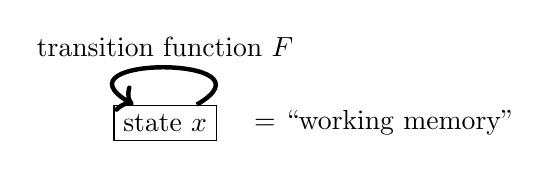
\begin{tikzpicture}[->]
\node[rectangle,draw,label=0:{{$\quad =$} ``working memory"}] (C) {state $x$};
\path (C) edge [out=30,in=150,looseness=4,ultra thick] node [above] {transition function $F$} (C);
\end{tikzpicture}
\end{equation}
When we add a ``control'' or ``action'' variable $a$ to it, it becomes the most basic  \textbf{control system}:
\begin{equation}
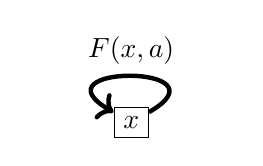
\begin{tikzpicture}[->]
\node[rectangle,draw] (C) {$x$};
\path (C) edge [out=30,in=150,looseness=7,ultra thick] node [above] {$F(x, a)$} (C);
\end{tikzpicture}
\end{equation}
which is the setting for Dynamic Programming or \textbf{Reinforcement Learning}.  The optimal solution for such systems is governed by the \textbf{Hamilton-Jacobi-Bellman equation}.

I call this the ``standard model'' because of the extreme simplicity of this setup, and that I don't know of other alternative models that deviate much from it.

%\section{The standard model in relation to other systems}

The following diagram shows how the standard model relates to several other important areas, so we can reap profits from their interactions:
\begin{equation}
\vcenter{\hbox{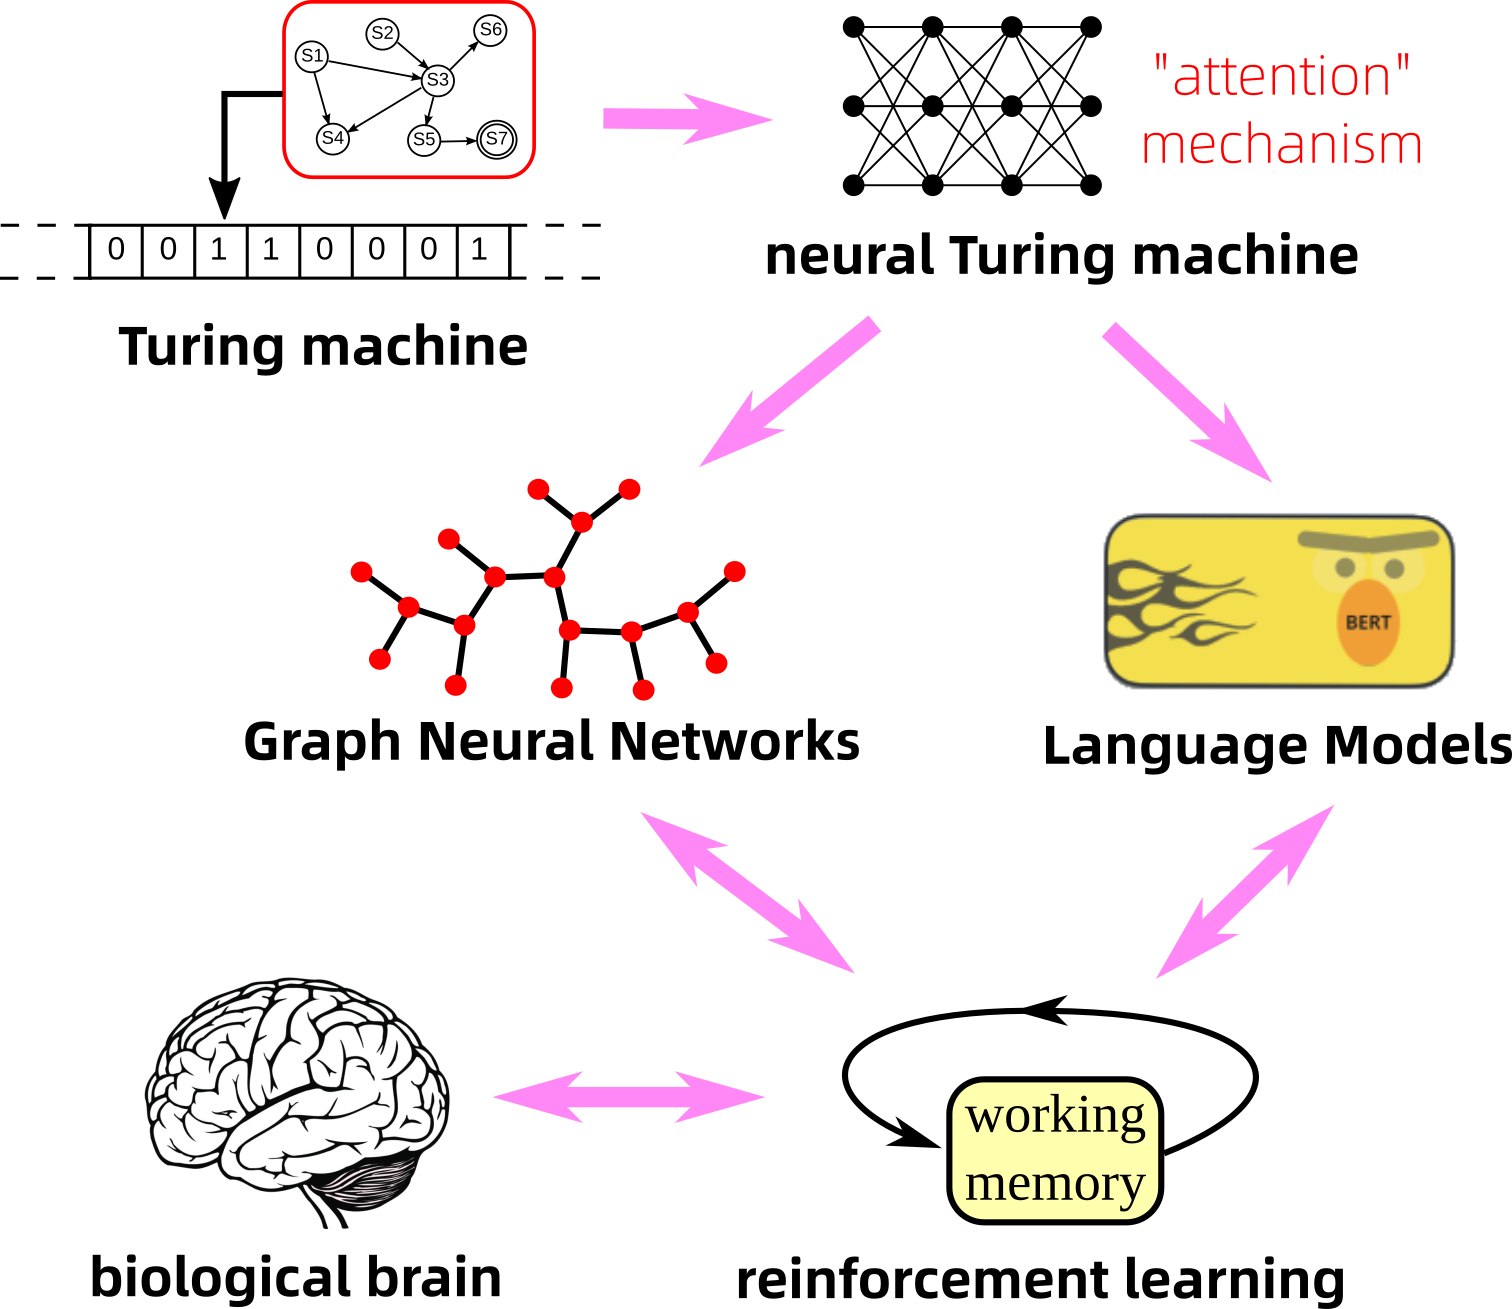
\includegraphics[scale=0.8]{AGI-standard-model.png}}}
\end{equation}

Recently, Yann LeCun's \textbf{Energy-Based Models} offers a way to circumvent the problem of learning probability distributions over actions, when the action space is hugely high-dimensional.

\section{Neural Turing Machines and Transformers}

The \textbf{attention mechanism} was first proposed in the ``\textbf{Neural Turing Machine}''  paper by Graves \textit{et al} [2014].

Recall that a Turing machine is a \textbf{Finite State Machine} augmented with a \textbf{Memory Tape}:
\begin{equation}
\vcenter{\hbox{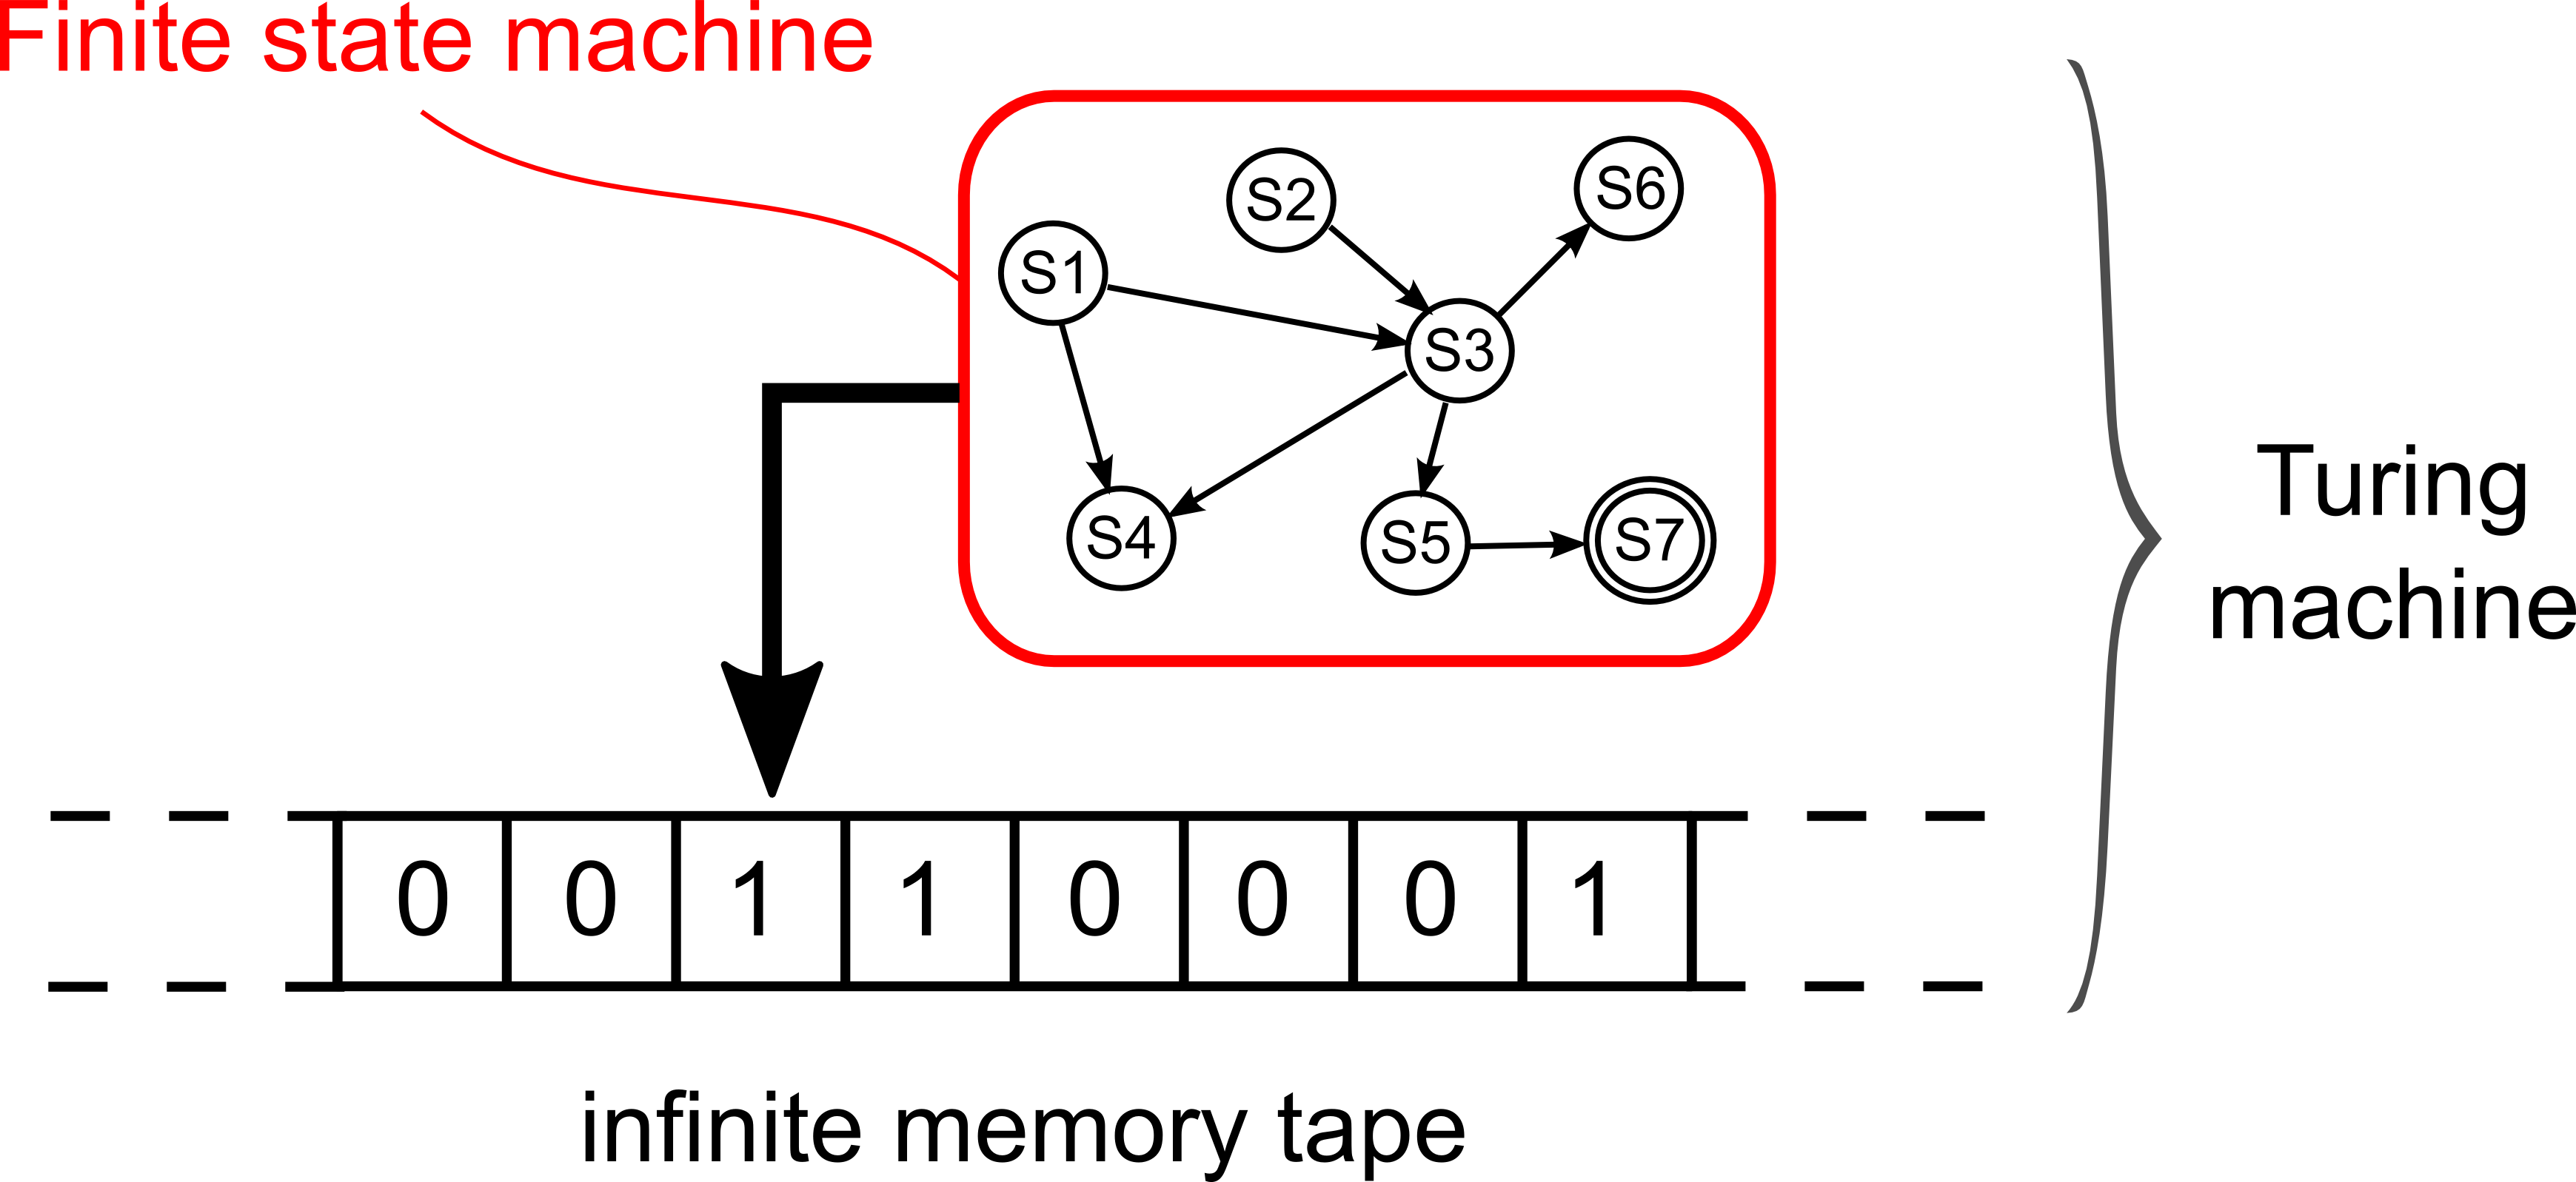
\includegraphics[scale=0.9]{Turing-machine.png}}}
\end{equation}

In Neural Turing Machines, Graves \textit{et al} proposed the attention mechanism for an RNN ``Controller'' (playing the role of the Finite State Machine) to read and write from a \textbf{Memory Matrix} (the tape), using a content-based addressing method.

The Memory Matrix $M$ consists of $N$ items, each of constant size.  \textit{The discreteness of the address would introduce discontinuities in gradients of the output}, hence we need an \textbf{Attention Vector} to focus on a specific location in the memory matrix $M$.

The Attention Vector $\vec{a}$ is calculated via the following formula, familiar to students of the Transformer: 
\begin{equation}
\vec{a} = \mathrm{soft} \max_i \{  \mathcal{D}(K, M_i) \}
\end{equation}
where $D()$ is a similarity measure between the key $K$ and memory item $M_i$.  The key $K$ is emitted by the Controller as the value that it is looking for.

This then evolved into the \textbf{Self Attention} mechanism used in all Transformers.  Now let us refresh with this diagram illustrating Self-Attention (ripped from a blog article on the web):

\begin{equation}
\vcenter{\hbox{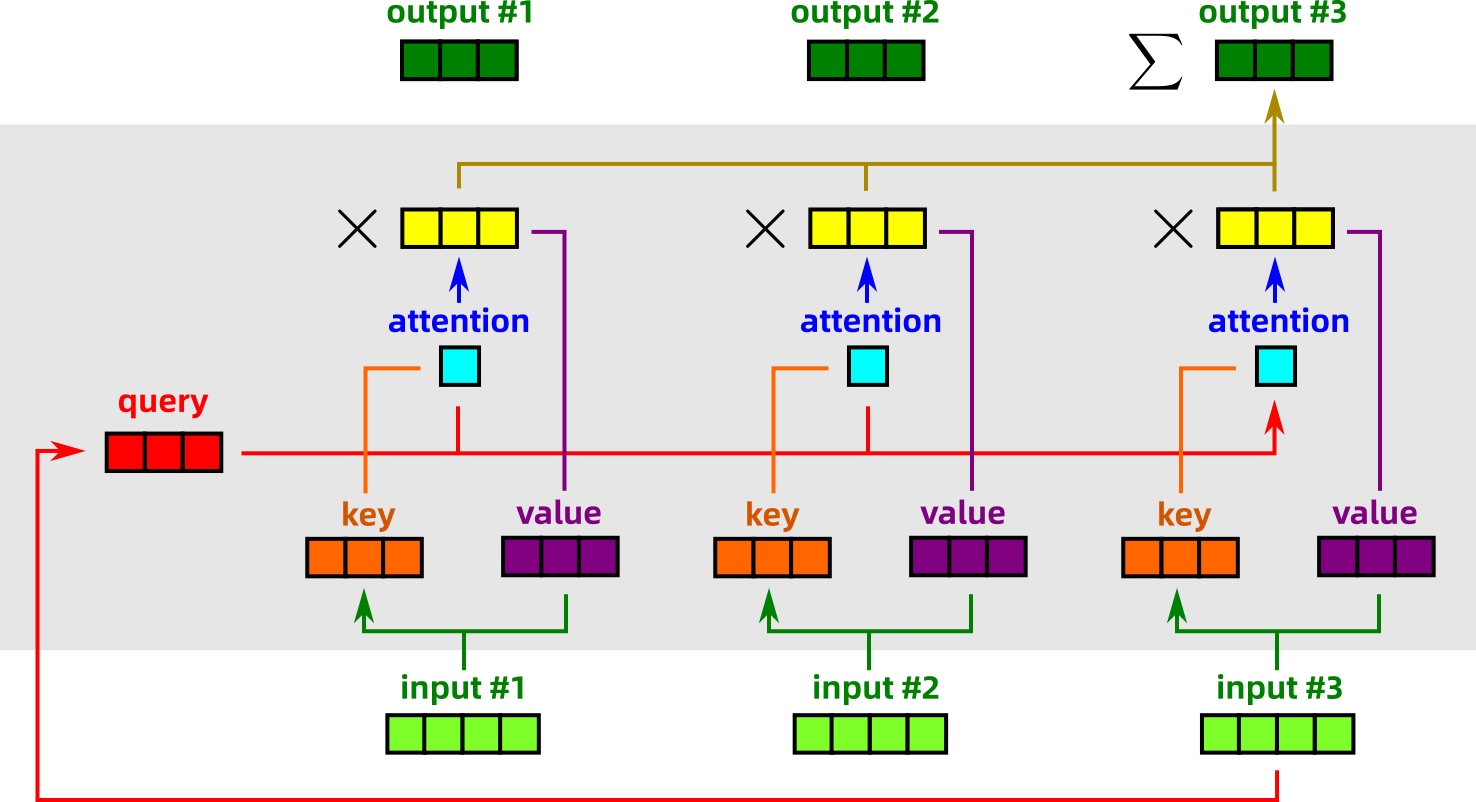
\includegraphics[scale=0.9]{self-attention-2.png}}}
\end{equation}

The research done by Olah \textit{et al}, in their 2021 paper \textit{\uline{A Mathematical Framework for Transformer Circuits}}, is very helpful towards understanding Transformers and Self-Attention.  The paper is technically quite challenging, but thanks to the guidance of professor Xiao Da from Beijing I was able to understand the main ideas.  Here I offer some pointers to help others understand the paper, without explaining it in full details.

The Self Attention $A$ is calculated by matrix operations followed by \textbf{softmax}, and thus is non-linear.  However, when $A$ is held constant, the Transformer becomes a linear operation that can be expressed as \textbf{tensor products}, for example:

\begin{equation}
\label{eqn:circuit1}
\vcenter{\hbox{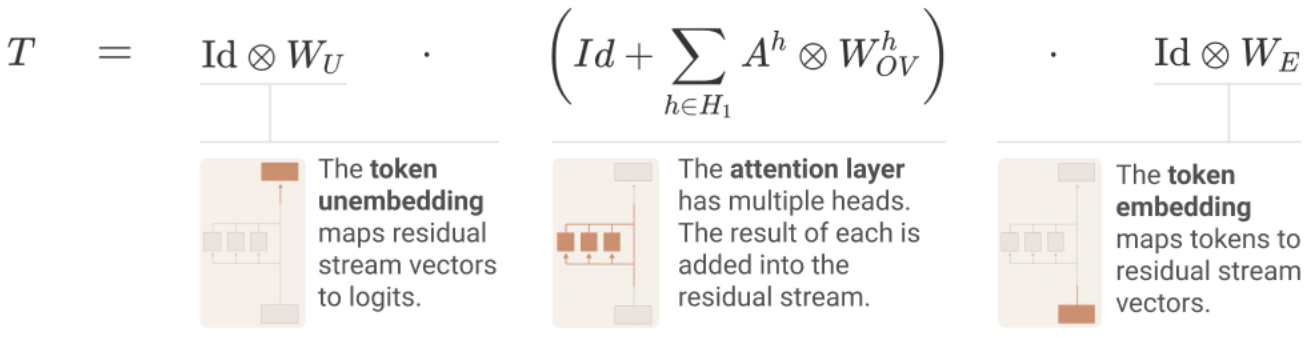
\includegraphics[scale=0.4]{Transformer-circuit-1.png}}}
\end{equation}

For example, to understand the equation for a Transformer ``Head'':
\begin{equation}
h(x) = (\text{Id} \otimes W_O) \cdot (A \otimes \text{Id}) \cdot (\text{Id} \otimes W_V) \cdot x
\end{equation}
it is helpful to know that $x$ is a \textbf{matrix} with dimensions $[n_{\mathrm{context}}, d_{\mathrm{model}}]$, ie, one dimension being the number of tokens and the other dimension representing the token's vector.  When a tensor such as $U \otimes V$ acts on $x$, $U$ acts on the ``position'' dimension of the matrix while $V$ acts on the ``vector'' dimension.  So the above equation can be collapsed to:
\begin{equation}
h(x) = (A \otimes W_O W_V) \cdot x .
\end{equation}
Thus tensor products are very convenient for expressing such operations.

\begin{tcolorbox}[breakable, parbox=false, fonttitle=\bfseries, title=Tensor product]
	
	Recall that a \textbf{linear} map is defined between two vector spaces:
	\begin{equation}
	F: U \rightarrow V .
	\end{equation}
	Similarly one can define a \textbf{bi-linear} map:
	\begin{equation}
	\Phi : V \times W \rightarrow U
	\end{equation}
	that is linear in both its first and second arguments.  The tensor product $\otimes$ is the \textbf{universal} multi-linear map.
	
	The tensor product generalizes to the mathematically important \textbf{monoidal categories}.  The latter captures the associativity (and optionally commutativity, for which we have symmetric monoidal categories), but the linearity is abstracted away.
	
	Monoidal categories can be depicted by \textbf{String Diagrams}.  There are also \textbf{Neural String Diagrams} that describe the structure of neural networks.  For example, the Transformer layer is \textbf{equivariant} in its inputs.

\end{tcolorbox}

In the Transformer, we can see \textbf{Input Values} flowing through some ``circuits'' defined by matrices to yield the \textbf{Output Values}:
\begin{equation}
\vcenter{\hbox{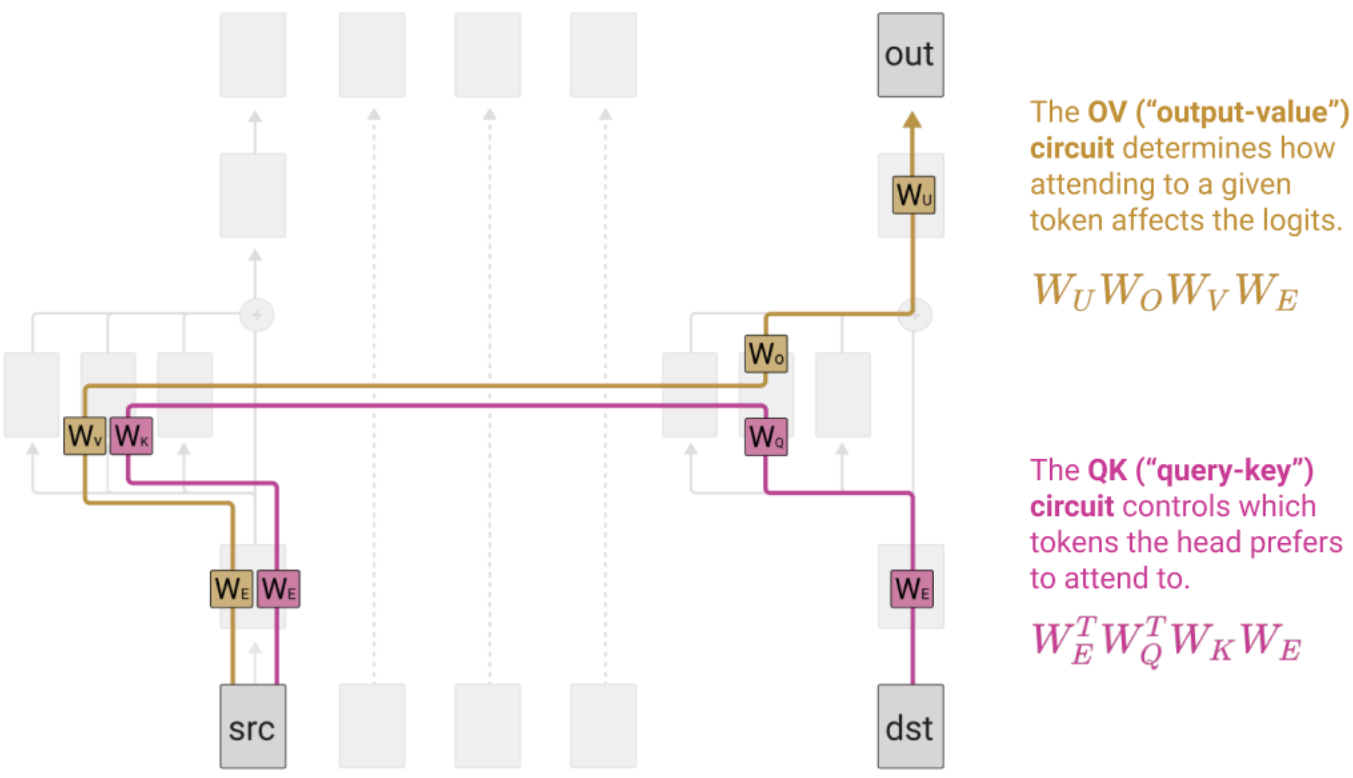
\includegraphics[scale=0.4]{Transformer-circuit-2.png}}}
\end{equation}

Some Attention Heads merely perform ``\textbf{copying}'' of a vector from a previous layer to the next.  If we spell this out as a linear equation, $W \vec{x} = \lambda \vec{x}$, where the transformation $W$ merely results in a \textbf{scaling} of the vector $\vec{x}$.  This is just an eigenvector equation.  So if we plot the eigenvalues of the transformation matrices on the complex plane, the ``copy'' maps would have eigenvalues close to positive real numbers.  The results shows that such ``copy'' maps are ubiquitous in Attention Heads (here 10 out of 12 maps are positive):
\begin{equation}
\vcenter{\hbox{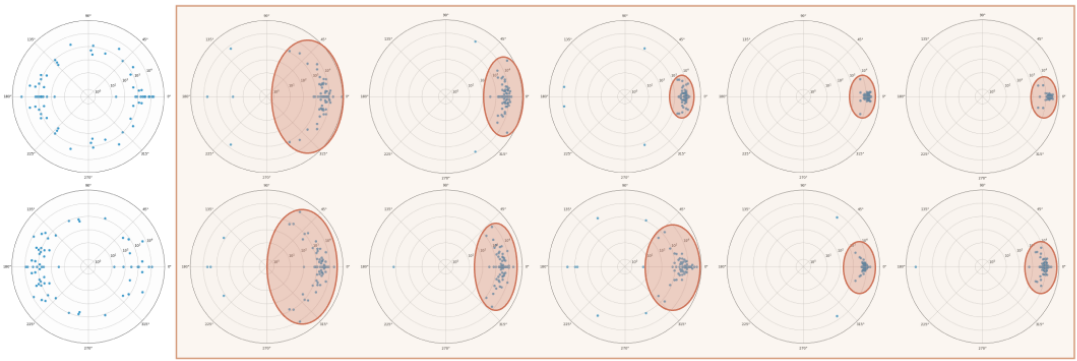
\includegraphics[scale=0.47]{eigenvalue-plot-of-Attention-Heads.png}}}
\end{equation}
Such Attention Heads may be interpreted as \textbf{universally-quantified} ($\forall$) logic formulas.  For example when we say ``all men are mortal'':
\begin{equation}
\forall x. \; Human(x) \Rightarrow Mortal(x)
\end{equation}
any object instantiated as $x$ (eg. ``Socrates'') would have to be \textbf{copied} from the LHS to the RHS.

\section{Relation to the biological brain}

There are two distinct aspects in the brain:
\begin{itemize}
	\item \textbf{Short-term} or Working Memory is the \textbf{electric activation} of neuronal populations.
	\item \textbf{Long-term} memory is stored as \textbf{synaptic strengths}, established by synaptic formation and strengthening.  The transfer from STM to LTM is called \textbf{memory consolidation}.
\end{itemize}

One theory has it that the prefrontal cortex maintains a number of ``thoughts'' with sub-populations or, perhaps, with \textbf{micro-columns}.  These activated sub-populations are in competition with each other, through \textbf{lateral inhibition}.  The thought(s) that win are the thoughts we retain -- they ``make sense''.

\section{Abductive reasoning}

Abduction has been relatively neglected in AGI research, which had focused on forward inference.  Recently there is a call to study this important aspect.

In logic, abduction means finding the \textbf{explanation} for some known facts.  An explanation $E$ is simply some propositions that imply the known fact $F$, ie, $E \Rightarrow F$.  For example, why is Marilyn Monroe sexy?  That's because she has a pretty face, big boobs, and a big ass.  So, $E_1 \wedge E_2 \wedge .... \Rightarrow \mathrm{Sexy}$.  Those conditions \textbf{imply} she is sexy, and they are the \textbf{explanation} for her sexiness.

Why is abduction important?  For example, when a waitress says ``The Ham Sandwich left a big tip'', \textit{Ham Sandwich} here refers to the customer who ordered it (an example of metonymy).  The AI knows the plain facts such as that someone ordered a ham sandwich, and then it abduces that the most likely \textbf{interpretation} of the phrase ``Ham Sandwich'' is as the person associated with it.  This is the basis of \textbf{Abductive Interpretation of Natural Language} proposed by Jerry Hobbs:
\begin{equation}
\vcenter{\hbox{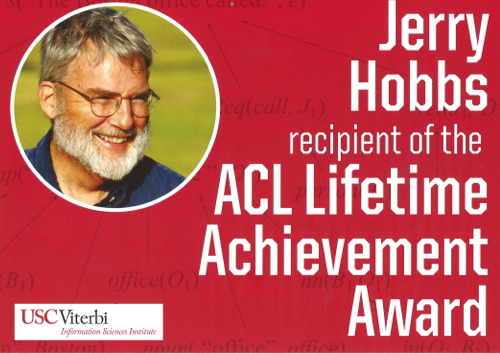
\includegraphics[scale=0.7]{Jerry-Hobbs.png}}}
\end{equation}

So abductive reasoning is basically just \textbf{bidirectional} inference.

When a system has both forward and backward connections, it forms a loop and its dynamics is likely to produce ``\textbf{resonance}''.  This harks back to the ART (\textbf{Adaptive Resonance Theory}) proposed by Grossberg and Carpenter beginning in the 1980s.

Such resonance behavior can be viewed as the system seeking to minimize an energy, ie, trying to find the ``best explanation'' to a set of facts.  

This is also corroberated by neuroscientific evidence:  areas in the cerebral cortex are replete with both forward- as well as \textbf{back-projections}.

\section{Dealing with assumptions}

Example of an assumption:  ``If I play move $x$ now, I will checkmate in 3 moves".

\begin{tcolorbox}[breakable, parbox=false, fonttitle=\bfseries, title=Tic Tac Toe example]
	
	Assume the current board is
	\scalebox{0.5}{
		\begin{tabular}{c|c|c}
			&     & \bO \\ \hline
			\bO & \Xb &     \\ \hline
			\Xb &     & 
	\end{tabular}} and it's \Xb's turn to play.
	
	\Xb \ can do the ``double fork'' by playing
	\scalebox{0.5}{
		\begin{tabular}{c|c|c}
			&     & \bO \\ \hline
			\bO & \Xb &     \\ \hline
			\Xb &     & {\color{red}\Xb}
	\end{tabular}}.
	
	But how can an AGI know (or prove) this?
	
	If the current board is 
	\scalebox{0.5}{
		\begin{tabular}{c|c|c}
			&     & \bO \\ \hline
			\bO & \Xb &     \\ \hline
			\Xb &     & \Xb
	\end{tabular}}  then a double fork exists.  We need a predicate to detect double forks.
	
	We need to reason that even if \ \bO \ plays the ``blocking'' move
	\scalebox{0.5}{
		\begin{tabular}{c|c|c}
			{\color{red}\bO} &     & \bO \\ \hline
			\bO & \Xb &     \\ \hline
			\Xb &     & \Xb
	\end{tabular}}  , \Xb \ can still win.
	
	We can easily express the conditions for \Xb-can-win, but the difficult part is to make the assumption in {\color{red}red}, in other words:
	\begin{equation}
	\mbox{{\color{red}red-move}} \rightarrow \mbox{\Xb-can-win}
	\end{equation}
	The difficulty lies in that the LHS is \textbf{not true} under the current facts.  This conditional statement must be proven by, first, assuming the LHS, and then deriving the RHS.  Then the assumption is \textbf{discharged} and the conditional statement is proven, via the ($\rightarrow$ I) rule.
	
\end{tcolorbox}

In the old days, in classical AI, assumptions are handled with \textbf{Truth Maintenance Systems} that keep track of inference traces symbolically.  These systems can get quite complicated with the need to track multiple assumptions.  For example, when we plan a bank robbery, we need to consider many possible forking scenarios.  

Suppose $M, N$ are proofs of $M: \phi \rightarrow \psi$ and $N: \phi$.  Then the proof of $\psi$ would be the application of $M$ to $N$, denoted as $@(M, N)$ or simply $M N$.

The assumption rule (Ax):
\begin{equation}
\Gamma, \phi \vdash \phi \qquad (\mbox{Ax})
\end{equation}
for example can be written as:
\begin{equation}
x : \phi, \; y : \psi \vdash x : \phi \qquad (\mbox{Ax})
\end{equation}
which is why we say that an assumption is a \textbf{$\lambda$-variable}.  

\textbf{Discharging} an assumption (ie, using the $\rightarrow$I rule) results in a \textbf{$\lambda$-term}.

An AGI needs the ability to place an implication $\phi \rightarrow \psi$ into working memory, and to prove it using the ($\rightarrow$ I) rule, ie, by making an assumption.

\textbf{Algorithm:}  Put the assumption $A$ in Working Memory.  Make inferences, marking all conclusions with the prefix $A \rightarrow *$.  When enough conclusions are obtained, remove the assumption $A$ from Working Memory.

\end{document}
